\subsection{Measuring risk}

Measuring risk and peoples behaviour under risky choice is a much debated topic in economics. In purely financial contexts variance is often used as a proxy for risk. Options with high variance are considered more risky than options with lower variance. 
A decision maker would therefore calculate the expected return and the corresponding variance of each option available.
Then if one option has lower risk and higher expected return than the other it is said to be dominant and should be preferred.
This model has some shortfalls, i.e. it is easy to construct cases where empirical studies clearly show that it is not sufficient to explain human behaviour.
% More complex measures have been introduced to explain these behaviours like Value At Risk, semi-variance (splitting variance into losses and gains) and expected shortfall. But all of these are highly abstract and would require quite some effort to evaluate as variance is hard to estimate. 
It can therefore be assumed that this hardly describes peoples everyday risk behaviour, instead a simpler and more intuitive way is required. \cite{Jaeger00}
% add example

Two mathematicians, Von Neumann and Morgenstern, gave rise to a method more useful for describing individuals behaviour. They postulated in the 1950s that when facing a risky decision people will maximize not their expected value but their expected utility. \cite{Morgenstern53}
The theory is therefore called expected utility theory.
To every possible outcome one assigns a utility value as defined by a real valued utility function. The person does not need to know (and most likely doesn't know) about their utility function. They will implicitly assign utilities and then pick the option that maximizes their expected function value.


\begin{figure}[ht]
\centering
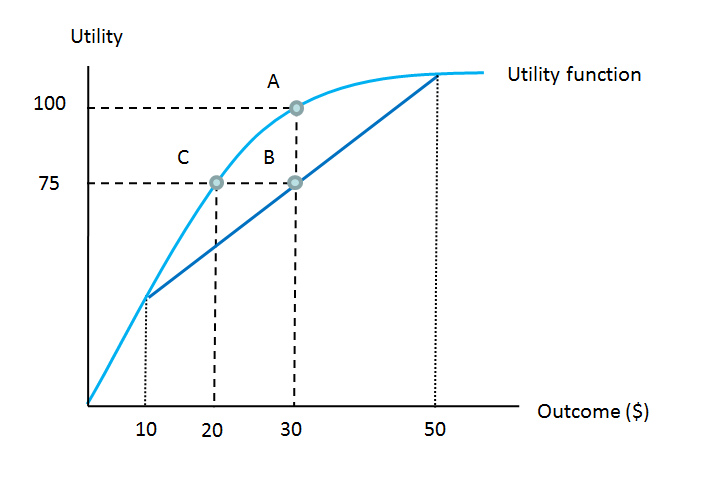
\includegraphics[width=0.5\textwidth]{img/background/riskaversion}%
\caption{Choice from a risk free gift of 30\$ or a lottery where by coin flip you win 10\$ or 50\$. The utility for the risk free choice (point A) is higher than the expected utility of the risky lottery (point B). 
% b) The exponential utility function for different risk parameters $\lambda$. $\lambda < 0$ implies risk seeking, $\lambda = 0 $ risk neutral and $\lambda > 0 $ risk averse behaviour.
}
\label{fig:background:riskaversion}
\end{figure}


To illustrate this we will look at the example illustrated in figure \ref{fig:background:riskaversion}:
A person is asked to choose from a gift of 30\$ or to participate in a fair coin flip where she can win 10\$ or 50\$.
It's easy to see that the expected outcome for both options is 30\$ but the coin flip is risky while the gift is risk free.
The person in figure \ref{fig:background:riskaversion} acts in line with a concave risk function, i.e. the utility grows slower than the outcome. This also leads to a saturation effect where higher values are valued less and less which can often be observed in economics. %https://books.google.de/books?id=II4Nwm1uoCIC&pg=PA156&lpg=PA156&dq=utility+saturation+effect&source=bl&ots=HTlYRm8HtH&sig=jlqdH5UPyURI-SWXYlCJ5DzWXsY&hl=de&sa=X&ved=2ahUKEwjL-cHox8bcAhWPZlAKHVj3DHMQ6AEwAXoECAEQAQ#v=onepage&q=utility%20saturation%20effect&f=false
The utility assigned to the possible outcome of 10\$ is around 40, the utility for 50\$ around 110 (both indicated by the dotted vertical lines). The expected utility of the coin flip (for different unfair coins) is simply the linear interpolation in between these two points. As we are using a fair coin the expected utility is right in the middle marked with the letter B at 75. In comparison the expected utility for the gift of 30\$ is at 100, indicated by letter A. The person in this example would therefore prefer the risk free choice of the gift over the risky coin flip.


\textbf{It is an important observation that concave utility functions describe risk averse decision makers whereas convex utility functions describe risk seeking decision makers. }

Different risk profiles can therefore be modelled by differently curved utility functions. Note that the curvature does not need to remain the same over all outcomes but can change, allowing to model risk seeking behaviour in some realm, e.g. for small amounts of money and risk averse behaviour in others, e.g. loss of life.

A very common and easy to parametrize utility function is the exponential function defined as:
\begin{flalign}
& U(w)  =  
\begin{cases}
	\frac{1-\exp(- \lambda w)}{\lambda} & \lambda \neq 0\\
	w & \lambda = 0
	\label{equ:exp}
\end{cases}
\end{flalign}
It is often chosen for its mathematical convenience yet its applicability is highly questionable as it implies time independent decisions, i.e. past losses are not considered when making new decisions. The impact of the parameter $\lambda$ on the curvature of the function is shown in figure \ref{fig:background:exponential}.

\begin{figure}[ht]
\centering
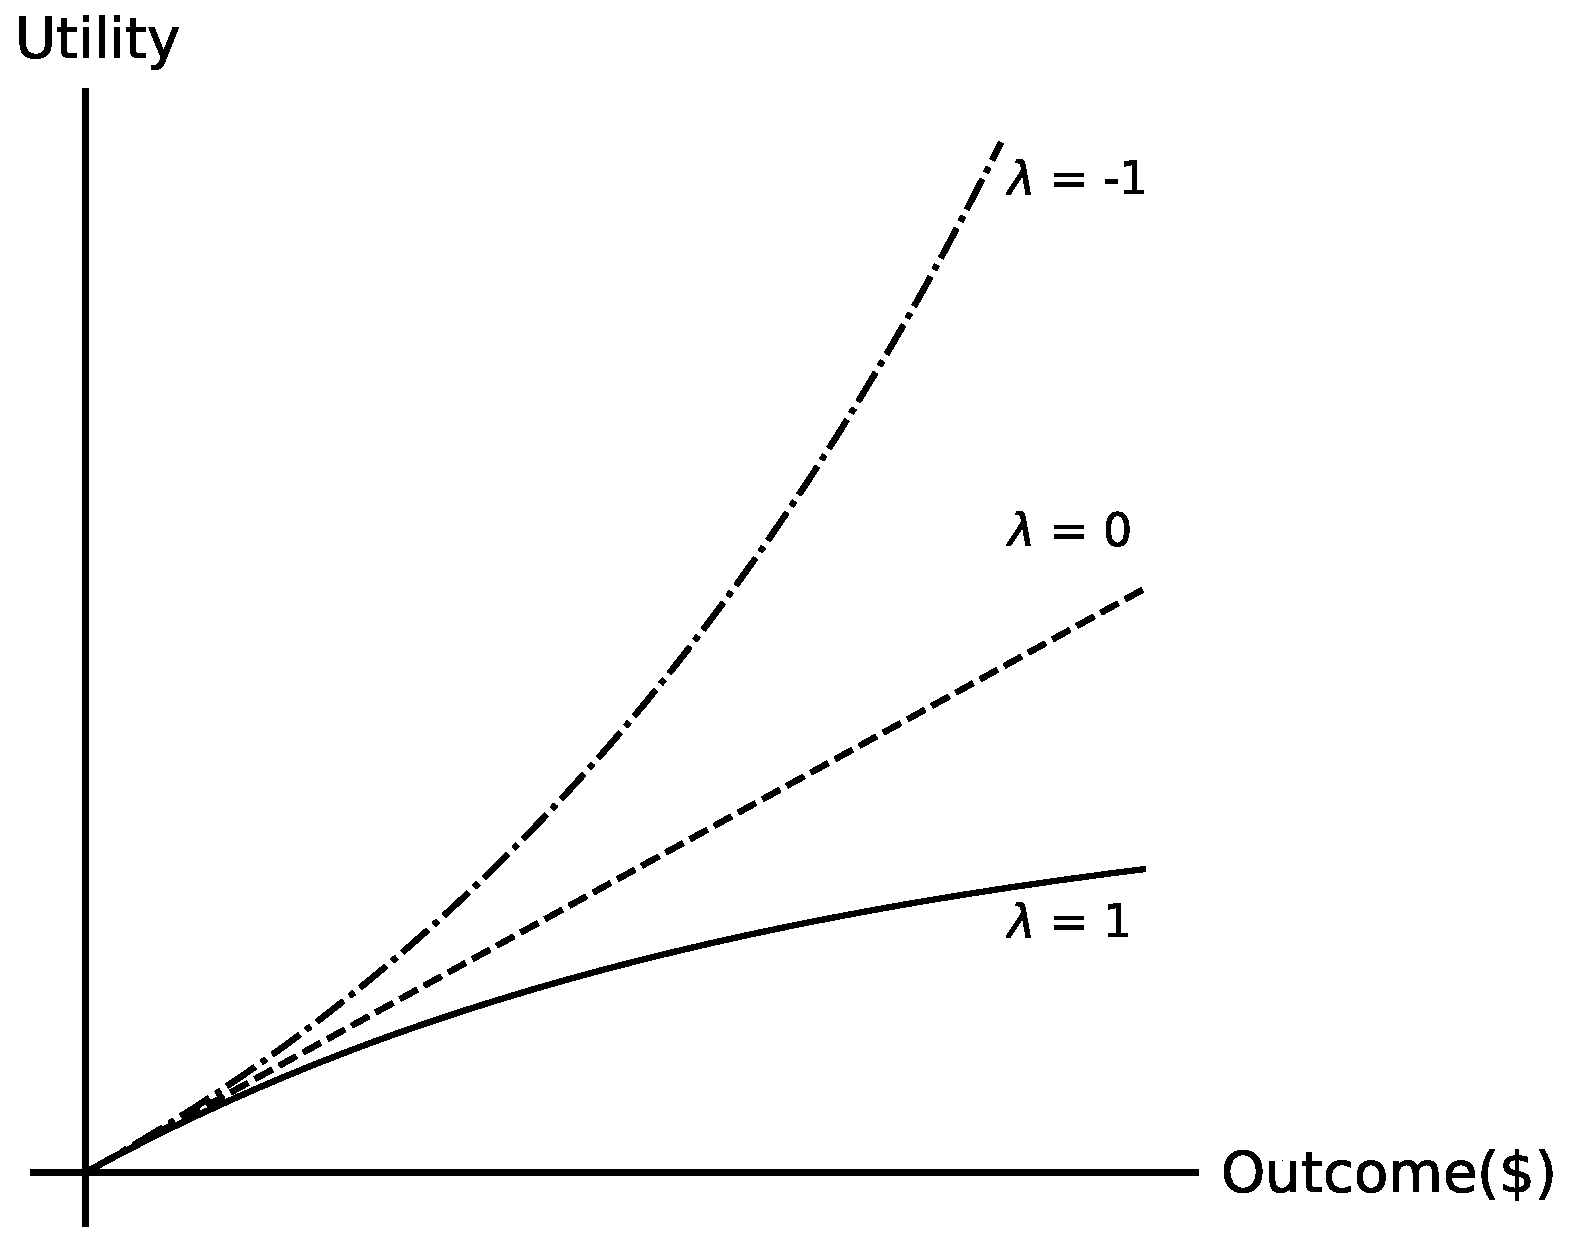
\includegraphics[width=0.3\textwidth]{img/background/Exponential_Utility_Function.pdf}%
\caption{ 
The exponential utility function for different risk parameters $\lambda$. $\lambda < 0$ implies risk seeking, $\lambda = 0 $ risk neutral and $\lambda > 0 $ risk averse behaviour.
}
\label{fig:background:exponential}
\end{figure}




% ###########################################################################

\subsection{Partially Observable Markov Decision Process}

Markov Decision Processes (MDPs) are a common choice for mathematically modelling risky decision making. Markov Decision Processes are usually defined over a finite state environment in which an agent can take actions with probabilistic outcomes that then affect the environment. At each time step the agent can fully observe in what state the environment is in.

Therefore an MDP is fully defined by the following four items:
\begin{itemize}
    \item Set of states $\mathcal{S}$ (terminal and non-terminal)
    \item Set of actions $\mathcal{A}$
    \item Probabilistic state transitions depending on tuple $\mathcal{S} \times \mathcal{A}$
    \item Reward function $R(s,a)$
\end{itemize}

To model decision making under uncertainty a MDP can be adopted to be partially observable instead. It is then called a Partially Observable Markov Decision Process (POMDP). In contrast to the classical MDP the agent no longer knows which state the environment is in. Instead it gets observations that it must use to infer the environments state.
This means the agent has to work on a probability distribution over states rather than the actual state.

To formally adopt the MDP framework we add two more items:
\begin{itemize}
    \item Observation space $\mathcal{O}$
    \item Observation function $p(o | s, a)$
\end{itemize}


A cartoon connecting all the pieces and showing the interactions between agent and environment can be seen in figure \ref{fig:background:agentenv}. The system is in a cyclical flow alternating between environment and agent. The agent performs an action that causes a state transition in the environment. The new state emits an observation and possibly a reward that are fed back to the agent. The agent uses this information to update its belief state and then acts according to its policy.

\begin{figure}
  \centering
    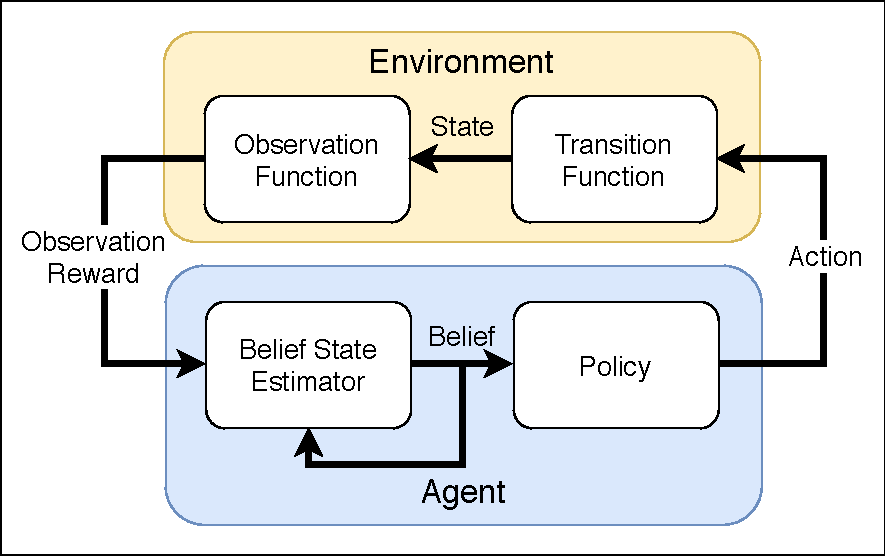
\includegraphics[width=0.5\textwidth]{img/background/POMDP}
  \caption{Sketch of a partially observable environment. The agent only gets observations and rewards as inputs but cannot see the state of the environment.}
  \label{fig:background:agentenv}
\end{figure}






% add reference: http://www.cassandra.org/arc/papers/aaai94.pdf
